% !TeX encoding = UTF-8
% !TeX program = pdflatex
% !TeX spellcheck = en_US

\documentclass[LaM,binding=0.6cm]{sapthesis}

\usepackage{microtype}

\usepackage{hyperref}
\hypersetup{pdftitle={Usage example of the Sapthesis class for a Laurea Magistrale thesis in English},pdfauthor={Francesco Biccari}}

% Remove in a normal thesis
\usepackage{lipsum}
\usepackage{curve2e}
\definecolor{gray}{gray}{0.4}
\newcommand{\bs}{\textbackslash}

% Commands for the titlepage
\title{A Large-scale Multi UAVs Reinforcement Learning Framework with Multiple Abstraction Layers}
\author{Giuseppe Capaldi}
\IDnumber{1699498}
\course{Engineering in Computer Science}
\courseorganizer{Facolt\`{a} di Ingegneria dell'informazione, informatica e statistica}
\AcademicYear{2019/2020}
\copyyear{2021}
\advisor{Prof. Luca Iocchi}
\advisor{}
\coadvisor{}
\authoremail{giuseppe.capaldi96@gmail.com}

\examdate{22 January 2021}	%TODO insert real data 
\examiner{Prof. Nome Cognome}
\examiner{Prof. Nome Cognome}
\examiner{Dr. Nome Cognome}
\versiondate{\today}
%====================================%====================================
%								MY PACKAGES
%%====================================%====================================
\usepackage{amsmath}

%%====================================%====================================

\begin{document}

\frontmatter

\maketitle

\dedication{Dedicated to\\ my family}

\begin{abstract}
Unmanned aerial vehicles (UAVs) are rapidly spreading in many different fields, setting new challenges, risks and opportunities in several real-life applications from civilian (surveillance, industrial monitoring, agricultural services, distaster relief, SAR) to military services (air exploration, battlefield surveillance, target localization, target tracking, target locking)\cite{Shakhatreh_2019}.\\
Among the application cases infrastructural inspection and damage assessment has been already be proven to be more efficient when using a UAV. More and more interest is growing in using group of UAVs to achieve higher efficiency, performance and resilience\cite{sysArch11}\cite{sysArch12}.\\
The use of multiple UAVs imposes the need of coordination and formation control when cooperating in solving a task of covering.
In the future multiple UAVs will coexist in the same large urban area, conducting different operations as single or group, probably without communication or cooperation among them.\\
In this context extending the view to a large-scale perspective, both in terms of number of vehicles and of space dimensions could be beneficial especially to mitigate the risk of collision. \\
Artificial intelligence and in particular Reinforcement Learning techniques could help in the choice of policies able to reduce these risks while optimizing in covering.\\
Virtual simulations can be used to find the best policies to be later tested and implemented in real life. \\
This master thesis will present methodologies, implementation and evaluations of a multi-layer framework based on multiple abstractions levels, aiming to transpose and improve existing Reinforcement Learning implementations to a 3D Realistic simulated environment.
In this sense the following projects could be considered as a solid starting point towards further developments.

The use of UAV will grow even more in the future and our cities will be impacted from the this considerable change.  
\end{abstract}

\begin{acknowledgments}
Ho deciso di scrivere i ringraziamenti in italiano
per dimostrare la mia gratitudine verso tutti coloro che mi hanno sostenuto in questo percorso accademico e di crescita personale.\\
Vorrei iniziare ringraziando il Prof. Luca Iocchi per avermi guidato con professionalit\'{a} e costanza, e per avermi affidato direttive chiare e utili allo sviluppo del progetto. \\
Sento di dover ringraziare anche i miei colleghi, in particolare Alessandro Trapasso e Federico Fiorini per il lavoro svolto assieme e il supporto morale.

Un ringraziamento va anche al Dott. Damiano Brunori che ha messo a disposizione la sua esperienza e il suo lavoro.

Infine una dedica speciale va fatta alla mia famiglia che non ha mai smesso di sostenermi.

\end{acknowledgments}

\tableofcontents


\chapter{Introduction}

\mainmatter
\chapter{Background} 
%(related work is a similar but different thing, in it you discuss also approaches that try solve similar problems)
\chapter{Methodology}

\section{Problem space}
%This section presents 
%TODO REMOVE%
(as a first draft)
a theoretical formulation of our problem, in which there are multiple UAVs sensing the simulated environment and sending data in real-time(images, GPS locations) to the ground station, making possible to train using reinforcement learning and optimize a fully cooperative task.  \\

One cooperative task could be defined as UAVs covering all the streets inside a controlled and bounded area, in the minimum possible time and avoiding collisions.
Covering means scanning through UAVs'on-board camera the street in search of targets. A target, that could be a 3D object (a car) or a 2D image (a bump in the road) is fully covered when it is seen fully by one camera from an angle.\\

This leads to several possible applications going from infrastructure inspections to surveillance of any kind.\\

Thanks to Unreal Engine editor the 3D map where the simulation is run can be customized to meet every need: from indoor to outdoor maps, including weather conditions, realistic textures and moving NPC (Non Playable Characters) as cars in traffic, moving animals or people. \\ % TODO insert some cite

For the conducted experiments two scenarios have been designed: a long road without intersections situated inside an highly realistic but fictional mountain landscape and a simplified (in terms of textures and general details)
urban environment that is a 1:1 scaled model of the real city, to be able to use real GPS coordinates. \\




\section*{Environment}
In the first scenario we can think of one or more targets, moving or stationary, that will be detected and classified, using standard supervised learning techniques (asynchronous calls to a specific thread), by a small number of UAVs. \\
Their navigation path will be determined by the results of the reinforcement learning training, in order to avoid collisions and minimize the time in which targets are detected, localized, classified.

\begin{figure}[hb!]
	\centering
	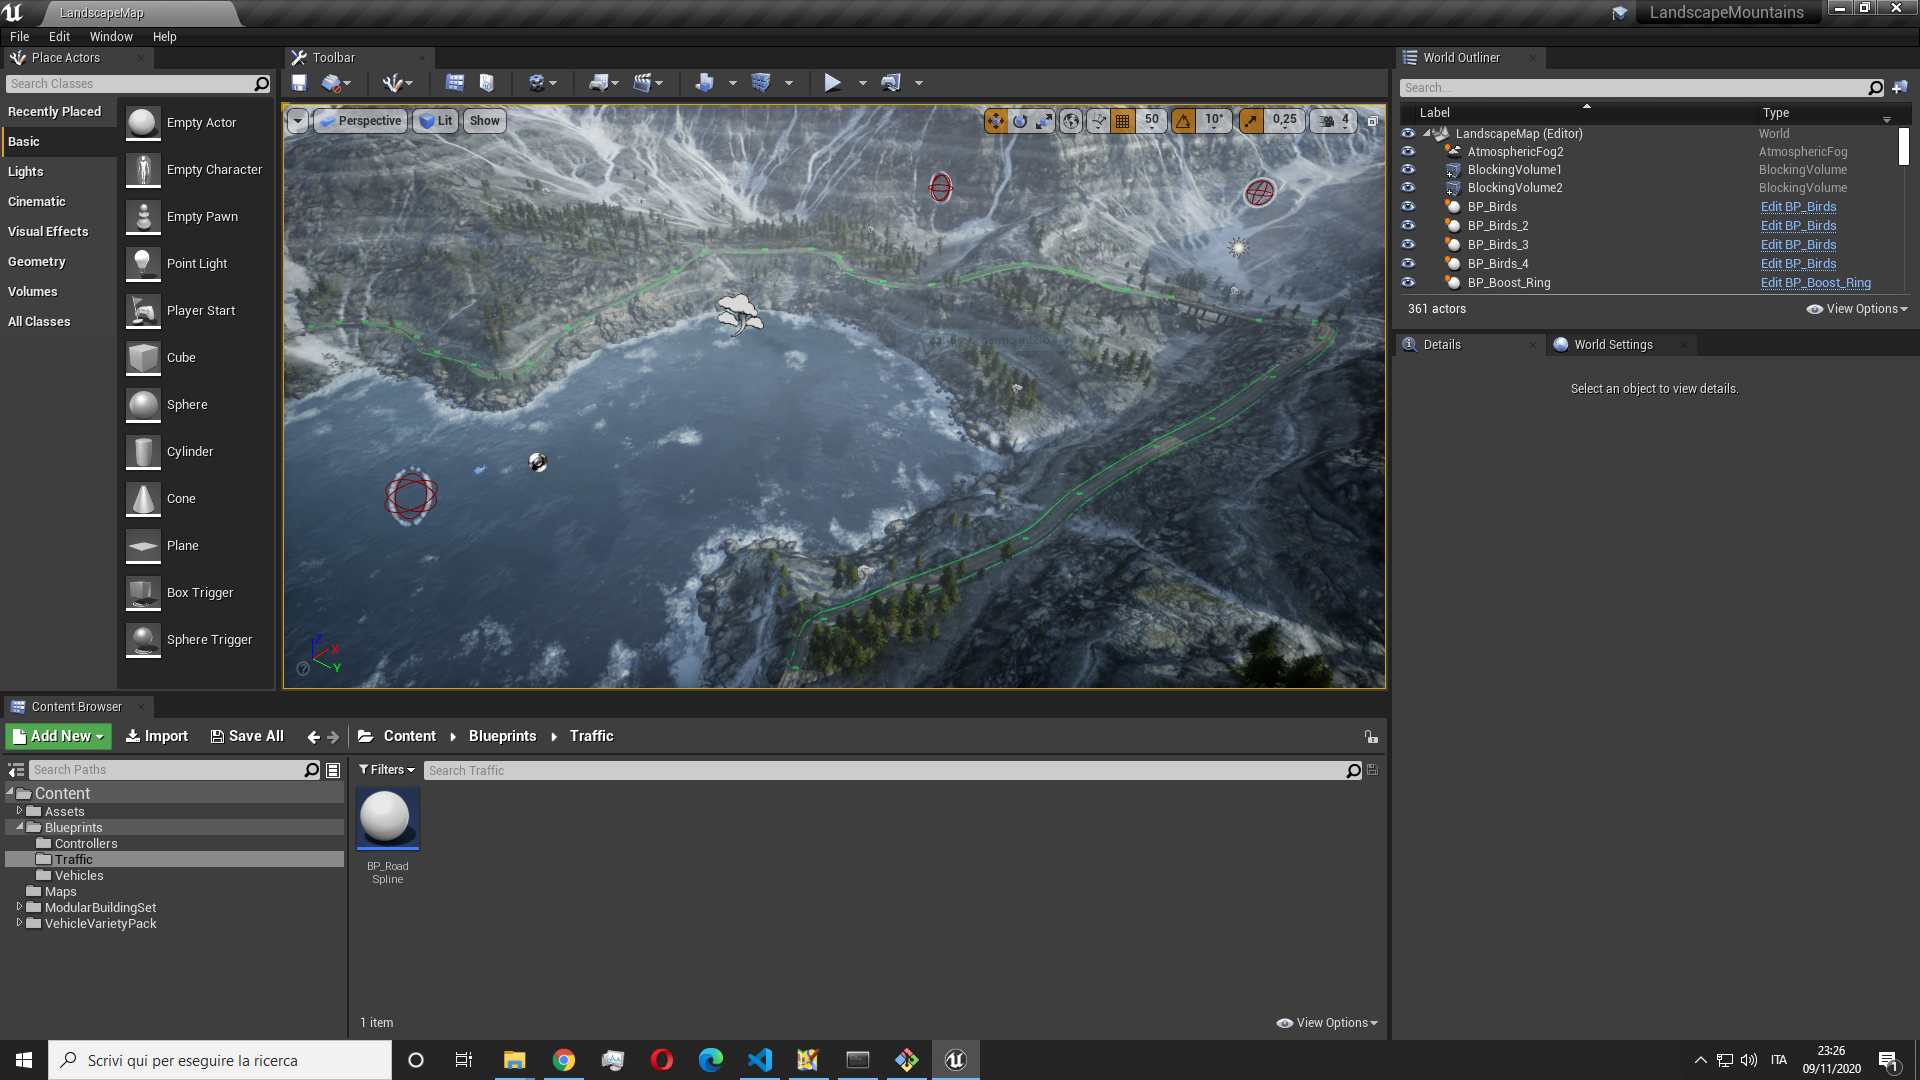
\includegraphics[width=1.0\columnwidth]{figures/Cattura6.PNG}
	\caption{Perspective view of the LandscapeMountain project. The green border delimits the border of the street.}
\end{figure}
\begin{figure}[!]
	\centering
	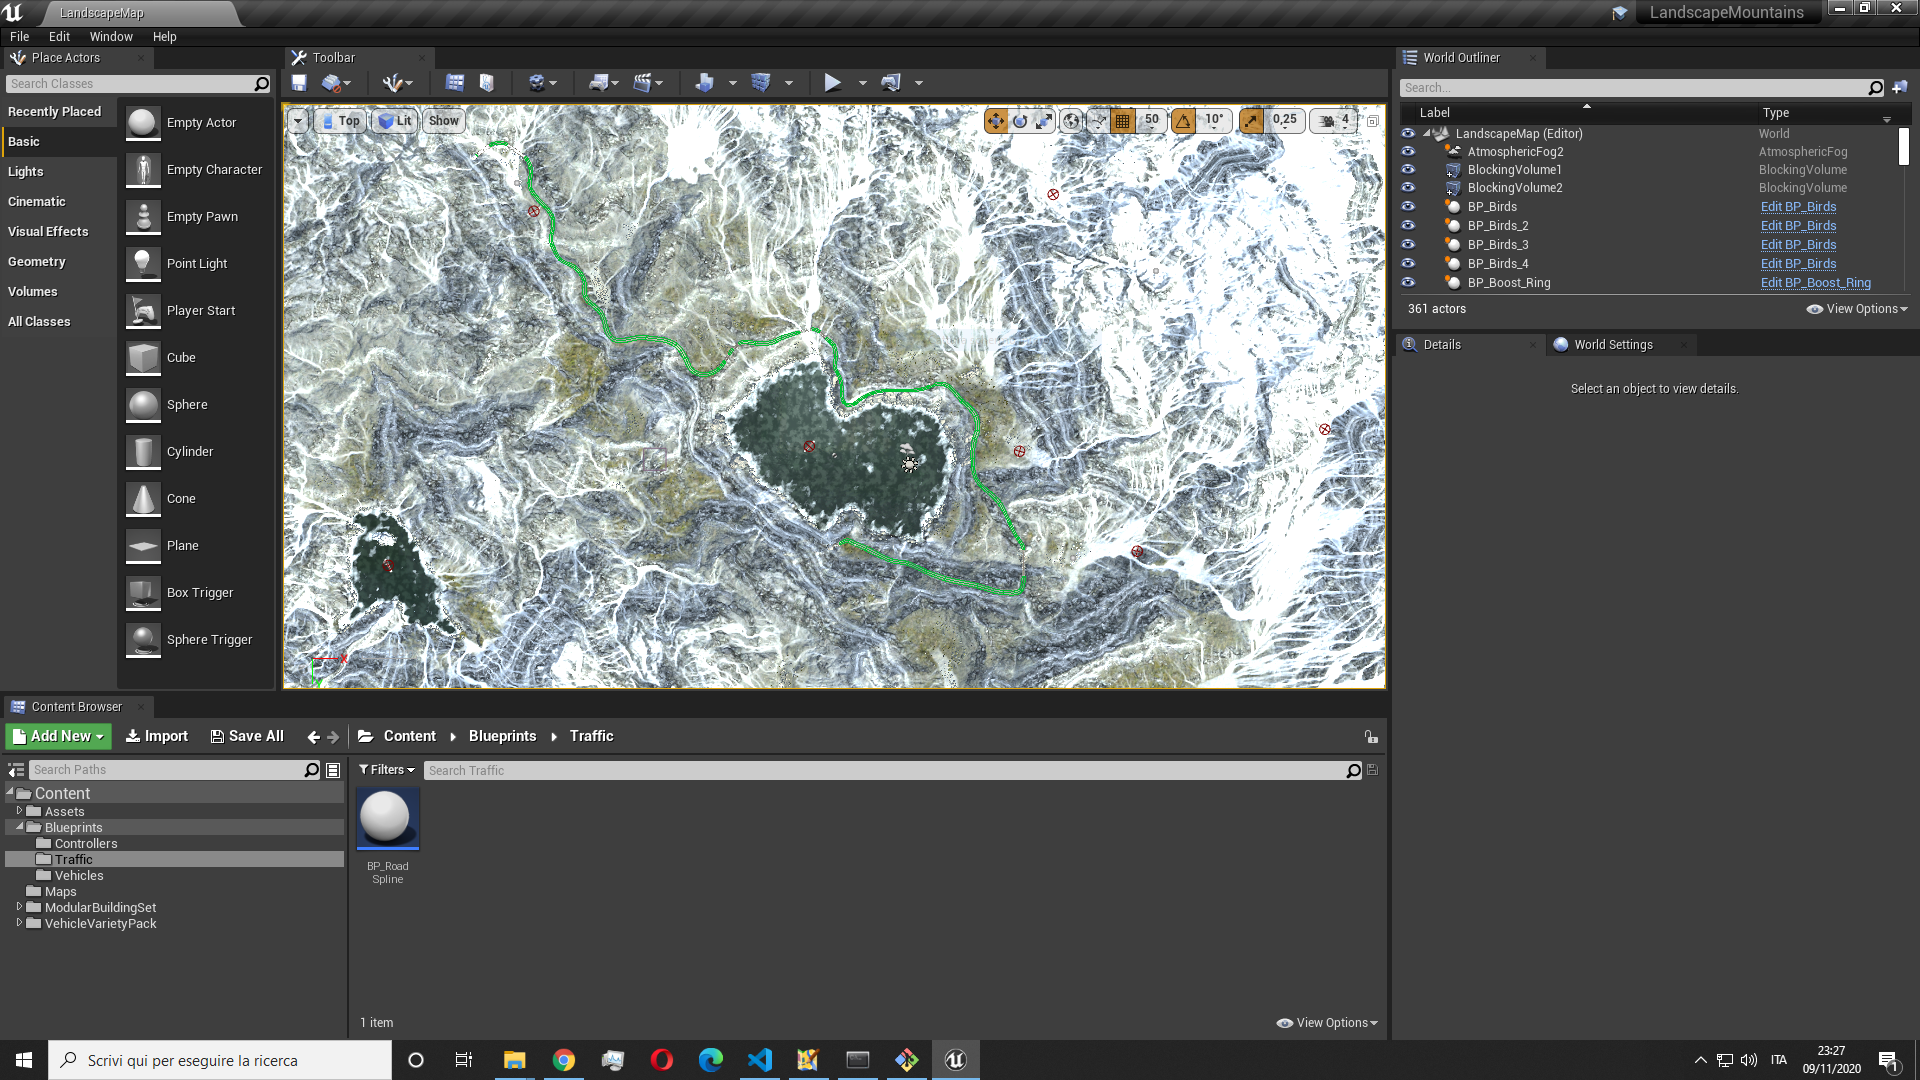
\includegraphics[width=1.0\columnwidth]{figures/Cattura7.PNG}
	\caption{Top view of the LandscapeMountain project. The green line represents the street.}
\end{figure}


The environment design is inspired by the free, but detailed and realistic "LandscapeMountains" Unreal project, which consists of a snowy mountain landscape with a long street crossing the entire map. The street has no intersection but it is not straight and some bridges sustain it in some areas.\\

In this scenario the Environment E consists of a non-flat space area of $E_x \times E_y$ meters. There are N agents (where $N\le6$) moving at the same discrete time synchronously, sending to the ground station at each time step information about the current state of drone $i$ at time step $t$.


The vehicles are assumed to be equipped with reliable
communication capabilities so that they can exchange sensing information among the group without any error or delay.
The objective of UAVs is to explore the environment cooperatively and to gather information till the target (or multiple targets) is detected and localized.\\
% 3D buildings
The second scenario provides for an environment $E$, considered as a non-flat space of dimension $E_x \times E_y$, with the presence of streets considerable as segment connecting GPS positions. 3D buildings are present as obstacles at the margin of the streets.\\
For this scenario too we can think of different initial positions for UAVs, this time they can be exctracted from a pool of possible initial positions costrained to be fairly distant one from the others.

Using GPS and Open data about the locations involved, we will use AirSim simulator to train on a map that will be generated from real data with 3D buildings and streets in the correct positions. GPS coordinates will be used to define paths over the streets (whose location is perfectly known) while 3D generated buildings will be useful to make realistic simulations of eventual collisions and visual obstructions in highly populated urban areas, exploiting the simulated cameras on the UAV.



\begin{figure}[hb!]
	\centering
	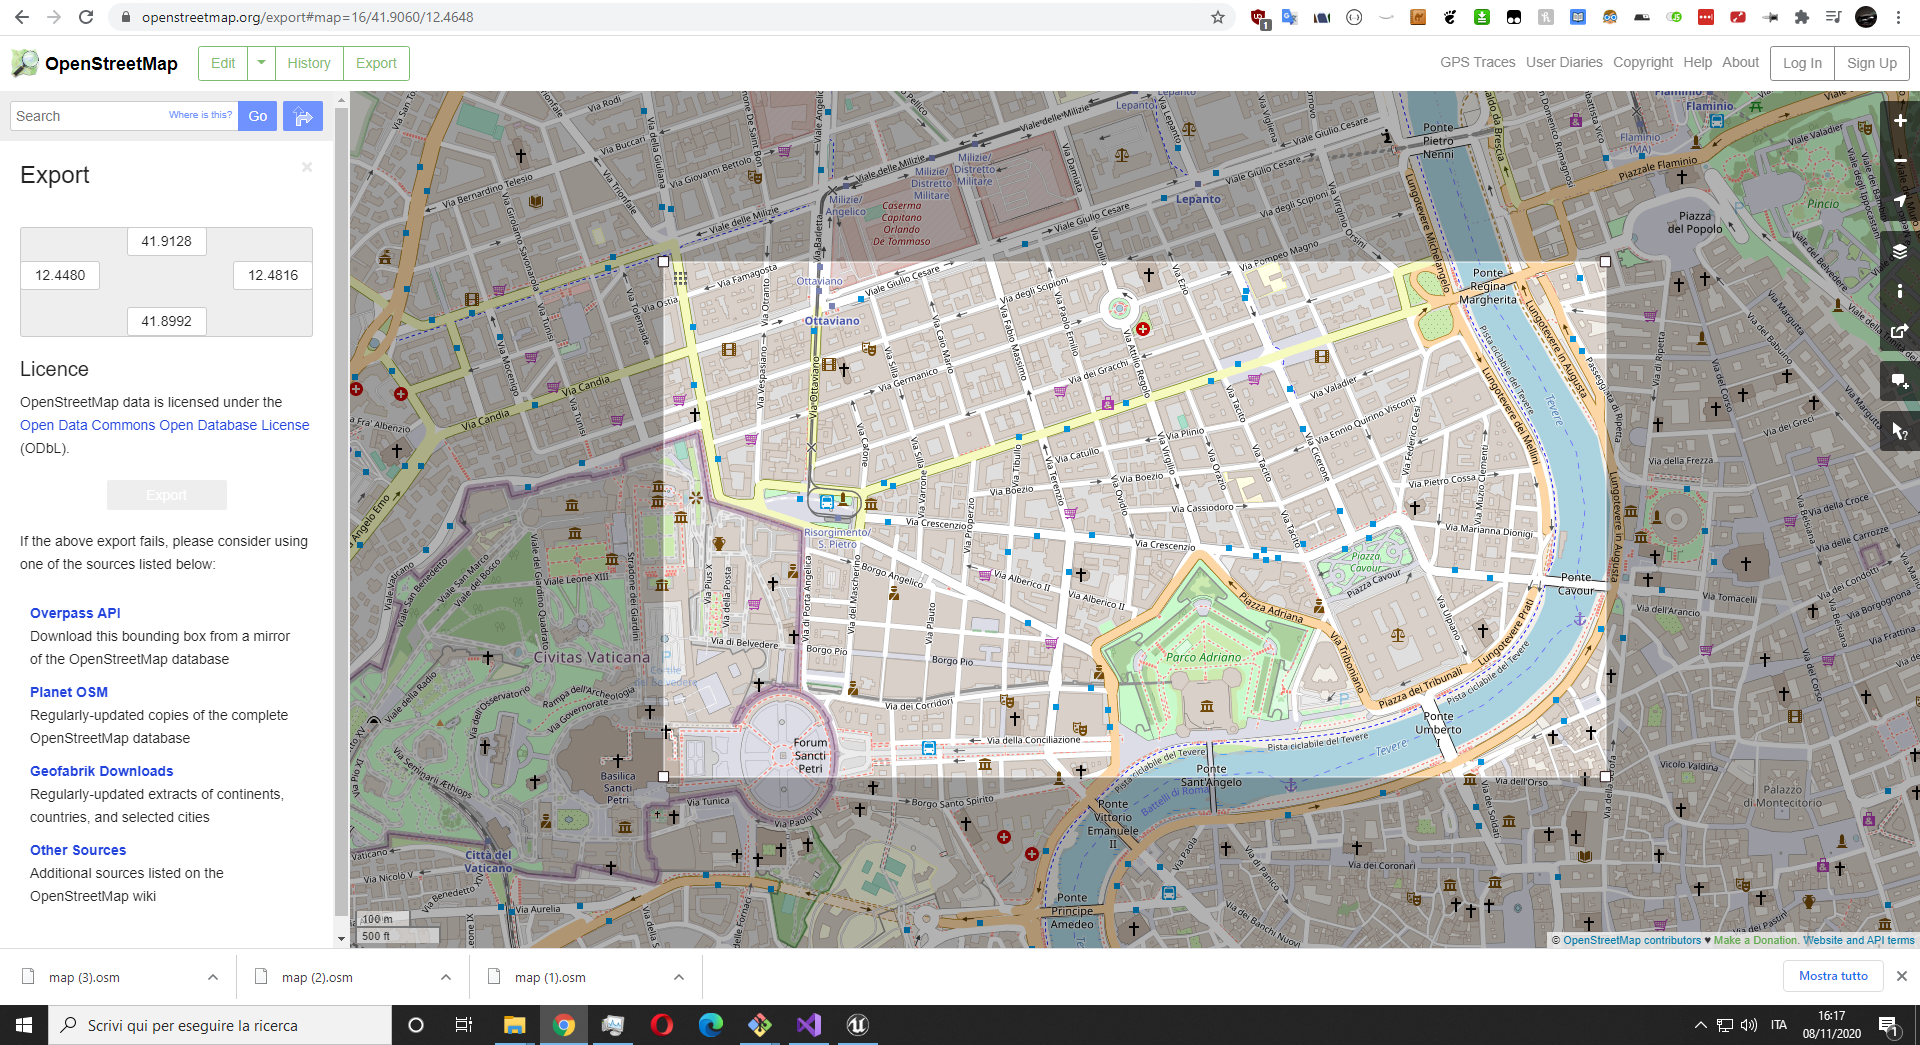
\includegraphics[width=1.0\columnwidth]{figures/Cattura3.PNG}
	\caption{OpenStreetMap website, it allows to download the .osm file to be later used as input to build 3D buildings assets.}
\end{figure}
\begin{figure}[!]
	\centering
	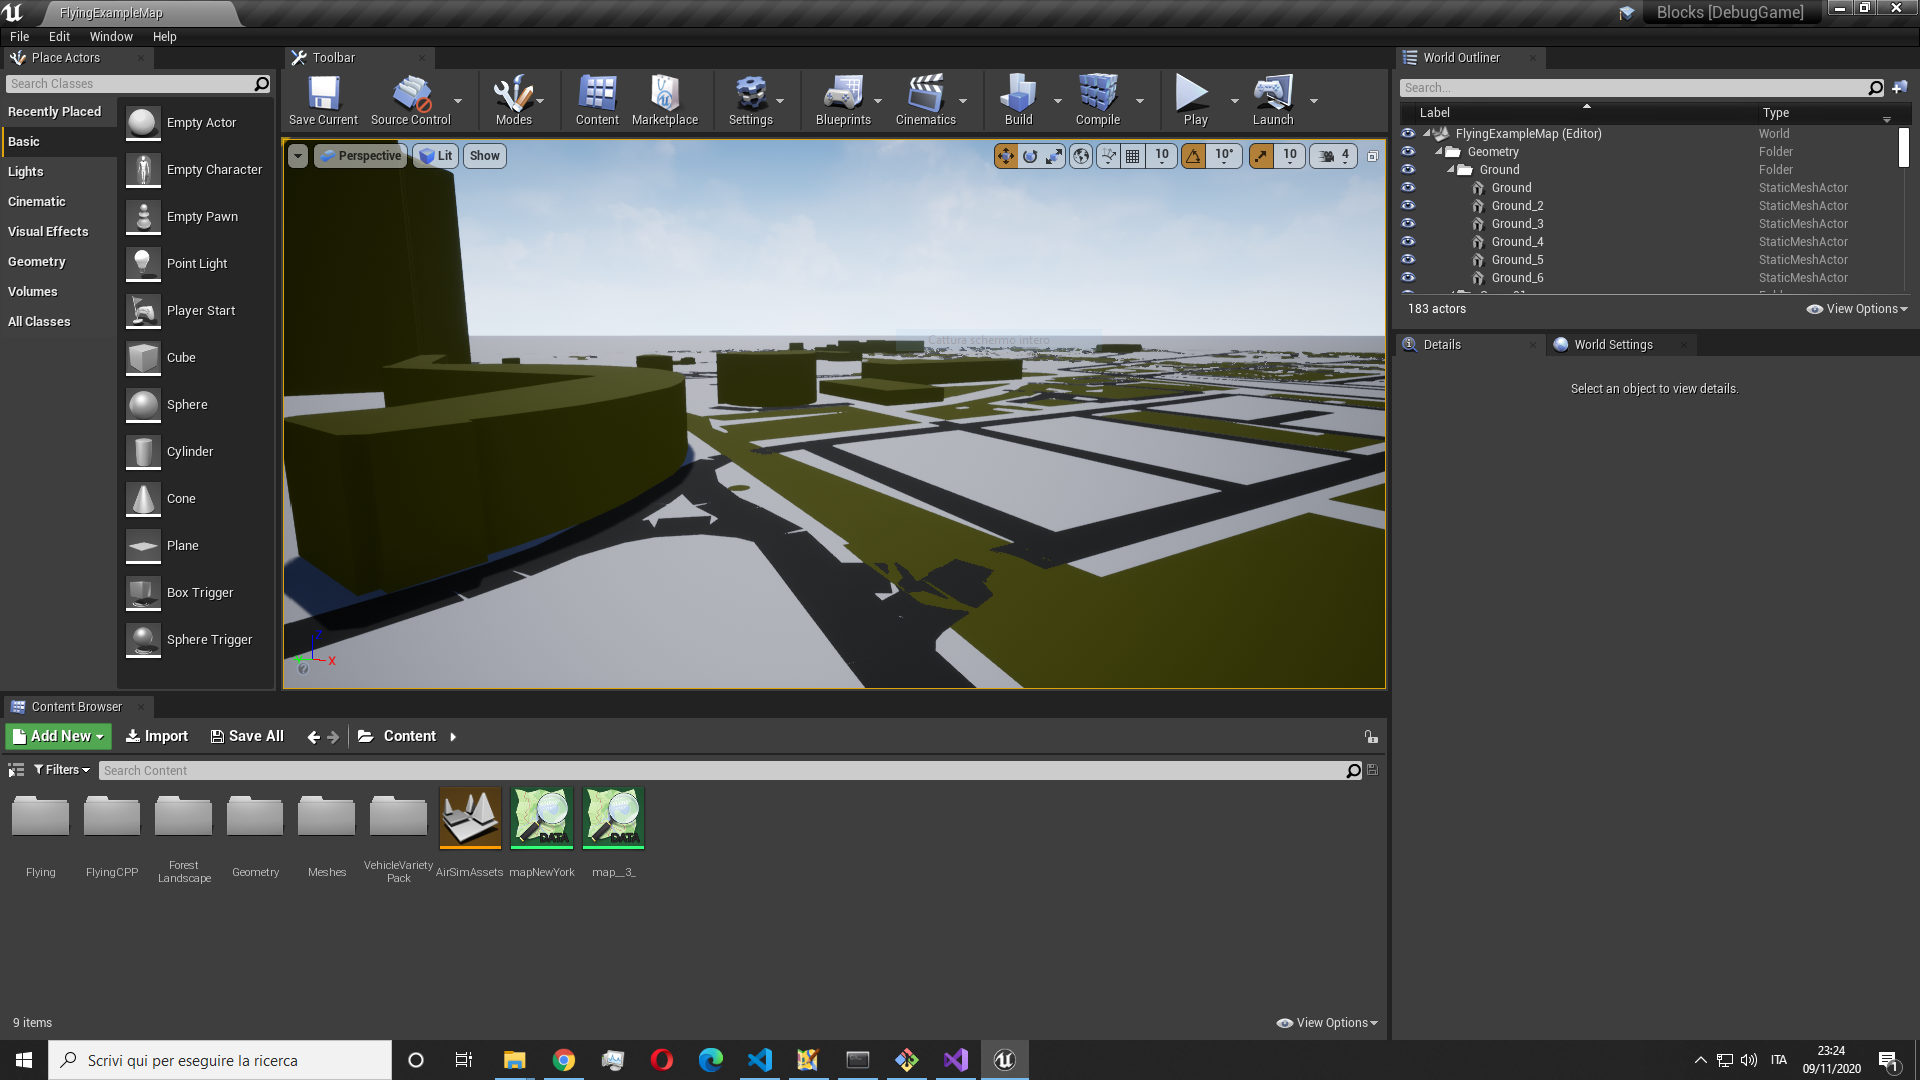
\includegraphics[width=1.0\columnwidth]{figures/Cattura5.PNG}
	\caption{Perspective view of the imported 3D assets map.}
\end{figure}


\subsection*{Action space for simplified Aerial Vehicle}
At initial timestep $t=0$ each UAV is laying on the ground, positioned inside the respective takeoff zone. Each UAV has associated a takeoff zone which is a rectangular area, not bordering with the others, used to delimit the random initial position for each single UAV inside of it.
% TODO specificare meglio %
At the next time steps each drone moves to the nearest point belonging to the line representing the street to be patrolled.
When a UAV is positioned over the street it start flying above it, so at each time step it moves and take pictures of the street. In this phase drones can move in 8 directions in order to follow the path of the street in both direction of travel. So the action space will be: 
$$ A = \{ 1 \mbox{ (up), }
2 \mbox{ (up-right), }
3 \mbox{ (right), } 
4 \mbox{ (down-right), }
5\mbox{ (down), }
6 \mbox{ (down-left), }
7 \mbox{ (left), } 
8 \mbox{ (up-left) }
\}$$
Each $a \in A$ has specific velocity and angles of motion designed to respect maneuverability constraints.

\subsection*{States and observations}
The state $s_i(t) \in S$ for vehicle $i$ at time step $t$ can be defined as so:
$$ s_i(t) = (\bar{g_{i}}(t),F_{i,t},C_{i,t})$$
where:
\begin{itemize}
	\item $\bar{g_{i}}(t) = (x_{i,t},y_{i,t},z_{i,t})$, $\bar{g_{i}}(t)$ are the GPS simulated coordinates at time $t$ for drone $i$, $x_{i,t}$ is the latitude coordinate, $y_{i,t}$ is the longitude coordinate, $z_{i,t}$ is the height
	
	\item $(F_{i,t})_{n\times m} = $ 
	$\begin{bmatrix}
	p_{0,0} & ... & p_{0,m-1} \\ ... & ... & ... \\ p_{n-1,0} & ... & p_{n-1,m-1} 
	\end{bmatrix}
	$, $F_{i,t} $ is a matrix of $n\times m$ pixels ($p$) taken by drone $i$ at time $t$
	
	\item $(C_{i,t})_{N\times N} = $ 
	$\begin{bmatrix}
	c_{0,0} & ... & c_{0,N-1} \\ ... & ... & ... \\ c_{N-1,0} & ... & c_{N-1,N-1} 
	\end{bmatrix}
	$,\\ \\
	$C_{i,t} $ is the communication matrix associated to instant t for drone i.\\
	$(c_{u,v})_{u,v=0,..,N-1} = \begin{cases} 0 \mbox{ (false)}, & \mbox{if } drone_{u,v} \mbox{ is outside coverage area of drone }i \\ 1 \mbox{ (true)}, & \mbox{otherwise}
	\end{cases}$
\end{itemize}. 
This information, in particular the first and last component ($\bar{g_i}(t)$ and $C_{i,t}$) are used to guide the search to certain areas of the
environment and can be consistently updated using sensor information about the environment. The communication matrix $C_{i,t}$ is used to prevent eventual collision and improve cooperation avoiding multiple exploration of the same places in a limited range of time.



\chapter{Implementation}
\chapter{Evaluation}
\chapter{Conclusion}

% Do not use the starred version of the chapter command!










\chapter{Style features of \textsf{sapthesis}}

In this chapter I will discuss my stylistic choices of \textsf{sapthesis}.
I will show the page layout geometry and I will describe the page style.

\section{Page layout}

The page is fixed at the dimensions of an A4 paper, therefore you have to print your thesis on A4 paper to obtain the best results. The font dimension is fixed at 11\, pt. The text column and the margins are chosen to fill to the best an A4 paper while keeping a reasonable line length (396\, pt) for a good readability. The text height and the text width are in golden ratio (\textasciitilde 1.6180) as well as the outer and inner margins in a two-side document after binding margin removal. Also the top margin (excluding the header) and bottom margin are in the golden ratio. In Fig.~\ref{layout} a sketch of the \textsf{sapthesis} page layout is shown.

\begin{figure}[h]
\centering
\setlength{\unitlength}{0.27mm}
\begin{picture}(420,297)(-210,0)
\polyline(-210,0)(210,0)(210,297)(-210,297)(-210,0)
\Line(0,0)(0,297)
\put(27.05,37.4){\polygon(0,0)(139.2,0)(139.2,223.8)(0,223.8)}
\put(-27.05,37.4){\polygon(0,0)(-139.2,0)(-139.2,223.8)(0,223.8)}
\put(27.05,268.16){\polygon(0,0)(139.2,0)(139.2,4.22)(0,4.22)}
\put(-27.05,268.16){\polygon(0,0)(-139.2,0)(-139.2,4.22)(0,4.22)}
\end{picture}
\caption{Page layout scheme of \textsf{sapthesis class} using a zero binding margin.}
\label{layout}
\end{figure}


\section{Page style}

The captions have a smaller font respect to the text and the label is in boldface. The appearance of the margin notes has been improved.
They have the same font dimension of the footnotes and are typed in italics.
Moreover I defined a new command to typeset margin note aligned to the left on the right page and vice versa on the left page.
Notice that if a binding margin greater than 1.5\, cm is used, the dimensions of the margin notes become too small and very ugly.
Do not use them in this case.

The mathematical objects, figures and tables are numbered within the chapters (e.g. 1.1, 1.2,\ldots for the first chapter, 2.1, 2.2 for the second one and so on\ldots). See for example the number of this simple equation
\begin{equation}
x_{1,2}=\frac{-b\pm\sqrt{b^2-4ac}}{2a}
\end{equation}


The title page is automatically composed when the \texttt{\bs maketitle} command is given.
The parameters needed for the title page, author, title, etc\ldots , are supplied by dedicated commands explained in the next section.
Two copies of the university logo in \texttt{pdf} format, one for color printing and the other one for black and white printing, are supplied in the \textsf{sapthesis} package. They are shown in Fig.~\ref{fig:largenenough}.

\begin{figure}
\centering
\includegraphics[width=0.7\textwidth]{sapienza-MLred-pos}\\[3ex]
\includegraphics[width=0.7\textwidth]{sapienza-MLblack-pos}
\caption{Logo of the Sapienza -- University of Rome.}
\label{fig:largenenough}
\end{figure}



\section{About figures and tables}

As regards the image formats, please use vector images as much as possible! Use jpg images only for photographs! pdf\LaTeX\ supports the pdf, jpg and png formats.

A very simple table is show in Tab.~\ref{tab:letters}. Remember to typeset
always the table caption above the table. Do not use vertical lines.

\begin{table}
\caption{This is a simple table.}
\label{tab:letters}
\centering
\begin{tabular}{lcc}
\toprule
Letter & Test & Test \\
\midrule
A & C & E \\
B & D & F \\
\bottomrule
\end{tabular}
\end{table}


\section{A section}

In this manual you can skip the gray text because it is just dummy text.

\textcolor{gray}{\lipsum[1-10]}



\section{Another section}

In this manual you can skip the gray text because it is just dummy text.

\textcolor{gray}{\lipsum}


\appendix
\chapter{Special commands provided by \textsf{sapthesis}}

\textsf{Sapthesis} provides some special commands, particularly useful for scientific works. You can use for example the roman shape, instead of the italic, for the imaginary unit (\texttt{\bs iu}) and Napier's number (\texttt{\bs eu}):
\begin{equation}
\eu^{\iu\pi}+1=0
\end{equation}

There are also two commands to speed up the writing of derivatives. In the following example we have used the commands \texttt{\bs der} and \texttt{\bs pder}):
\begin{equation}
\der{f}{x} \qquad \pder{f}{*{2}{y}}
\end{equation}


\textsf{Sapthesis} provides also 4 commands to improve the writing of subscripts, \texttt{\bs rb} and \texttt{\bs tb}, and superscripts, \texttt{\bs rp} and \texttt{\bs tp}. Two of these commands, \texttt{\bs rb} and \texttt{\bs rp}, can be used both in text and in math mode and compose their argument in roman. The other two, \texttt{\bs tb} and \texttt{\bs tp}, can be used only in text mode and compose their argument as are. Here it is an usage example of \texttt{\bs rb} and \texttt{\bs rp}:
\[
a_b \neq a\rb{b}\qquad a^b \neq a\rp{b}
\]
And here it is an usage example of \texttt{\bs tb}: \emph{Cu\tb{It} indicates copper bought in Italy}. And a usage example of \texttt{\bs ts}: \emph{Cher G\tp{le} Napol\'eon}.


Then several commands for the correct typesetting of unit of measurements are provided. For example the command \texttt{\bs un} typesets its argument in roman and leaves a thin space between the number and the unit: $25\un{m}$, $3.5\un{m/s}$. Other commands are: (\texttt{\bs g}) 45\g, (\texttt{\bs C}) 30\,\C, (\texttt{\bs A}) 12\,\A, (\texttt{\bs micro}) 40\,\micro m, (\texttt{\bs ohm}) 27\,\ohm. 

We have also \texttt{\bs x} as abbreviation of \texttt{\bs times}: \texttt{\$7 \bs x 10\^{}5\$} gives $7 \x 10^5$. Then \texttt{\bs di} is the differential symbol which automatically insert the correct spacing.
\[
\int x \di x
\]

Finally we have defined the color \textsf{sapred} which is the official color
of Sapienza -- University of Rome. It is defined as RGB(130,36,51). \textcolor{sapred}{This text is written with the color \textsf{sapred}.}

In the following dummy text you can observe the usage of \texttt{\bs mnote} command which typesets fancy margin notes.

\textcolor{gray}{\lipsum}
\marginpar{This is a fancy margin note!}
\textcolor{gray}{\lipsum}

\backmatter
% bibliography
\cleardoublepage
\phantomsection
\bibliographystyle{sapthesis} % BibTeX style
\bibliography{bibliography} % BibTeX database without .bib extension

\end{document}
